\documentclass[a4paper, 12pt]{article}

\usepackage{geometry}
\geometry{left=2cm, right=2cm, top=2cm, bottom=2cm}

\usepackage{cmap}
\usepackage{mathtext} 
\usepackage[T2A]{fontenc}
\usepackage[utf8]{inputenc}
\usepackage[english,russian]{babel}	

\usepackage{amsfonts,amssymb,amsthm,mathtools}
\usepackage{amsmath}
\usepackage{icomma} 

\usepackage{graphicx} 
\graphicspath{{picturies/}}
\usepackage{wrapfig}

\usepackage{array,tabularx,tabulary,booktabs}
\usepackage{longtable}
\usepackage{multirow}

\usepackage{caption}
\captionsetup{labelsep=period}

\renewcommand{\phi}{\varphi}
\newcommand{\eps}{\varepsilon}
\newcommand{\parag}[1]{\paragraph*{#1:}}

\newcounter{Points}
\setcounter{Points}{1}
\newcommand{\point}{\arabic{Points}. \addtocounter{Points}{1}}

\author{Радькин Кирилл, Б01-005}
\date{04.12.21}
\title{Лабораторная работа 3.4.5. Петля гистерезиса (динамический метод).}

\begin {document}

\maketitle

\parag {Цель работы} изучение петель гистерезиса различных ферромагнитных материалов в переменных полях.

\parag {В работе используются} автотрансформатор, понижающий трансформатор (или реостат), интегрирующая ячейка, амперметр и вольтметр (мультиметры), резистор, делитель напряжения, электронный осциллограф, тороидальные образцы с двумя обмотками.

\parag {Теоретическая справка} ~\\

К ферромагнетиками принадлежат железо, никель, кобальт, гадолиний, их многочисленные сплавы с другими металлами. К ним примыкают ферриты~--- диэлектрики со структурой антиферромагнетика.

Магнитная индукция $\vec{B}$ и напряжённость магнитного поля $\vec{H}$ в ферромагнитном материале неоднозначно связаны между собой: индукция зависит не только от напряжённости, но и от предыстории образца. Связь между индукцией и напряжённость поля типичного ферромагнетика на графике выражается петлёй гистерезиса (см. рис. \ref{gist}).

\begin{figure}[!h]
    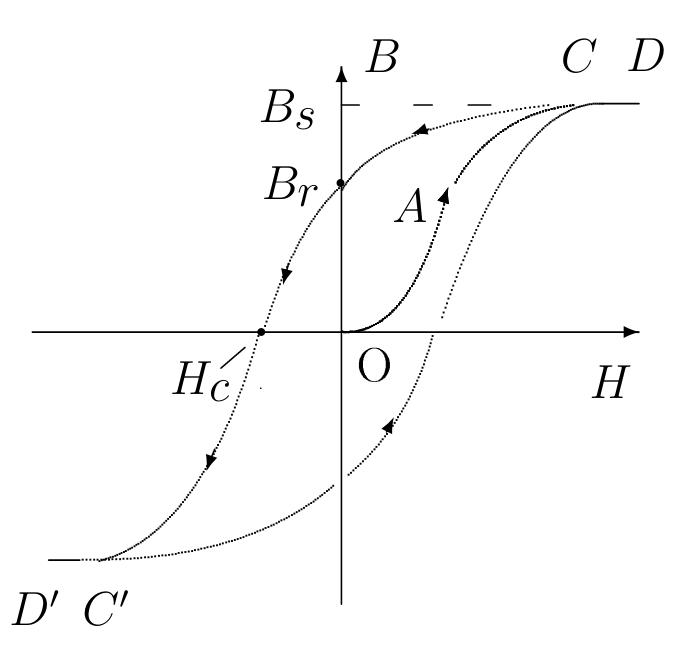
\includegraphics[scale = 0.2]{Gist}
    \centering
    \caption{Петля гистерезиса ферромагнетика}
    \label{gist}
\end{figure}

\parag {Экспериментальная установка} ~

Схема установки изображена на рис. \ref{workplace}. Напряжение от сети с помощью трансформатора $T$ подаётся на намагничивающуюся обмотку $N_0$ исследуемого образца.

Напряжённость $H$ в образце определяется по теореме о циркуляции с помощью эффективного значения силы тока $I_0$, измеряемого амперметром. Магнитная индукция $B$ с помощью интегрирующей RC-цепочки.

\begin{figure}[!h]
    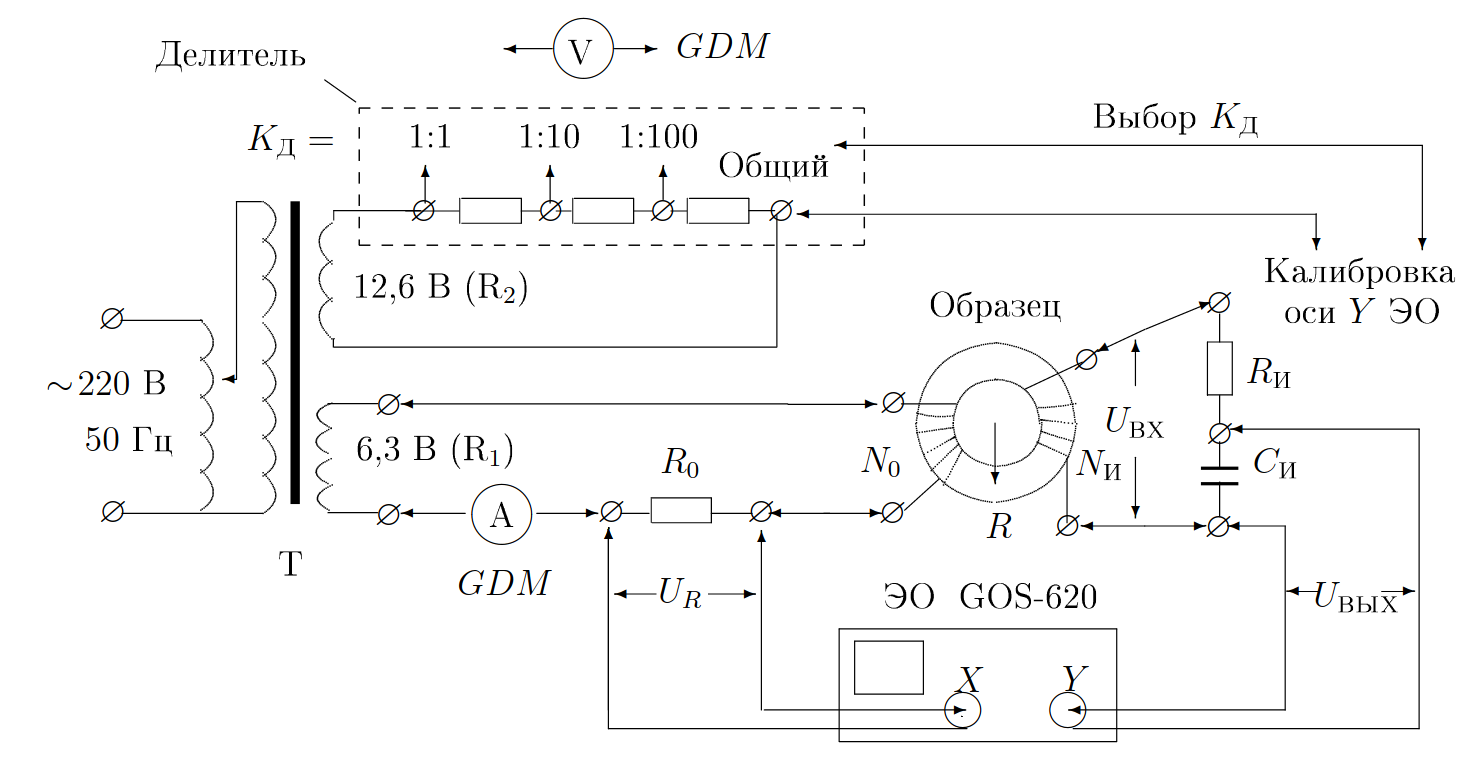
\includegraphics[scale = 0.2]{Workplace}
    \centering
    \caption{Схема установки для исследования намагничивания образцов}
    \label{workplace}
\end{figure}

\parag {Ход работы} ~\\

\point Для наблюдения петли гистерезиса на экране ЭО соберём схему согласно рис. \ref{workplace}. Подготовим приборы к работе. 

\point С помощью потенциометра подберём ток питания в намагничевающей обмотке так, чтобы на экране наблюдалась предельная петля гистерезиса. Подберём коэффициенты усиления каналов ЭО так, чтобы предельная петля занимала большую часть экрана. Сфотографируем и зарисуем на кальку предельную петлю и оси координат. Измерим все необходимые величины (согласно описанию работы). Нанесём кривую начального намагничивания.

\point Повторим предыдущий пункт для всех образцов (всего их 3: феррит, пермаллой (Fe-Ni) и кремнистое железо (Fe-Si)). Результаты см. на фотографиях кальки.

\begin{figure}[!h]
    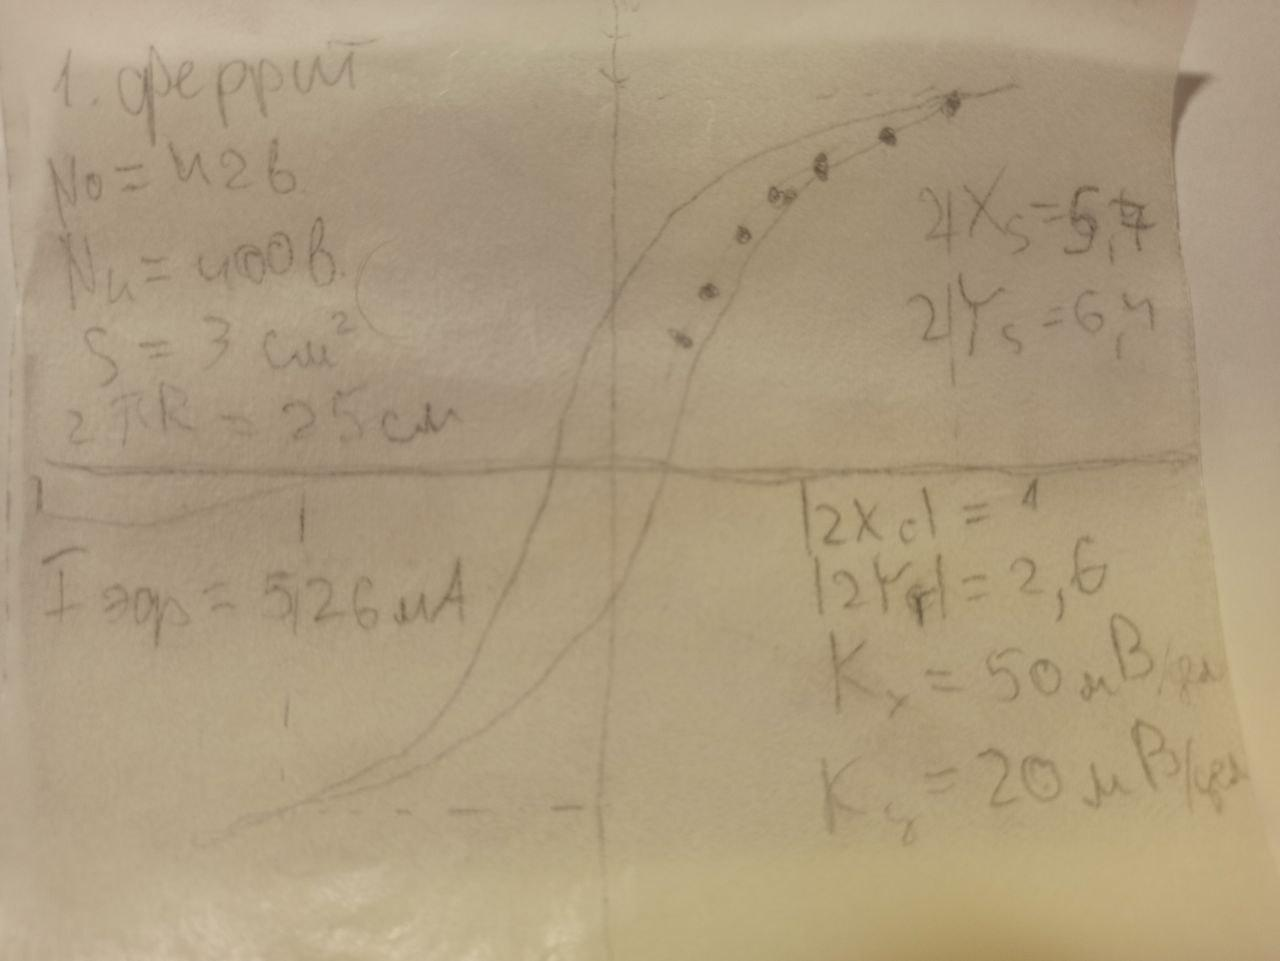
\includegraphics[scale = 0.15]{1}
    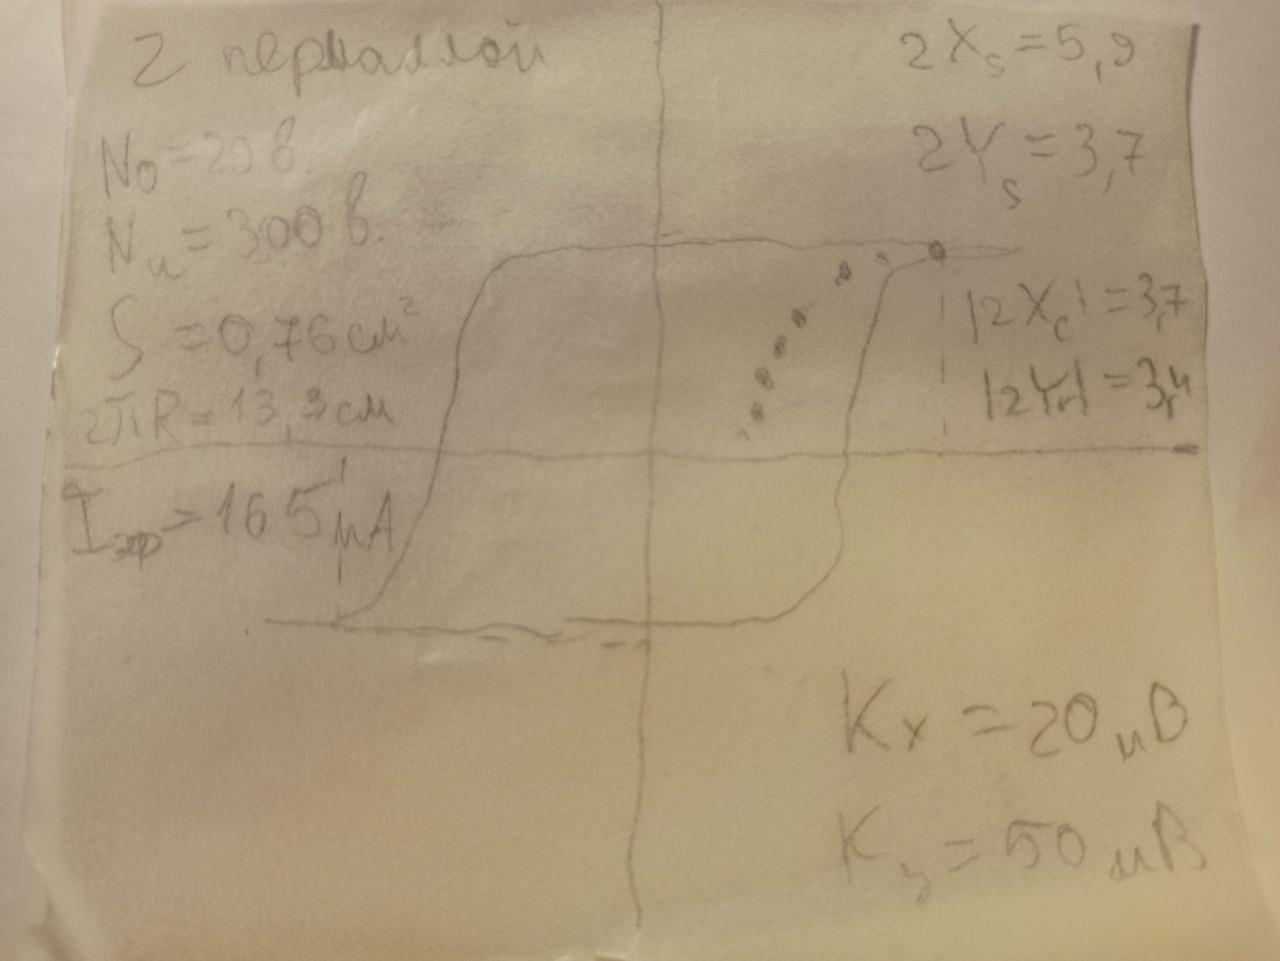
\includegraphics[scale = 0.15]{2}
    \centering
\end{figure}

\begin{figure}[!h]
    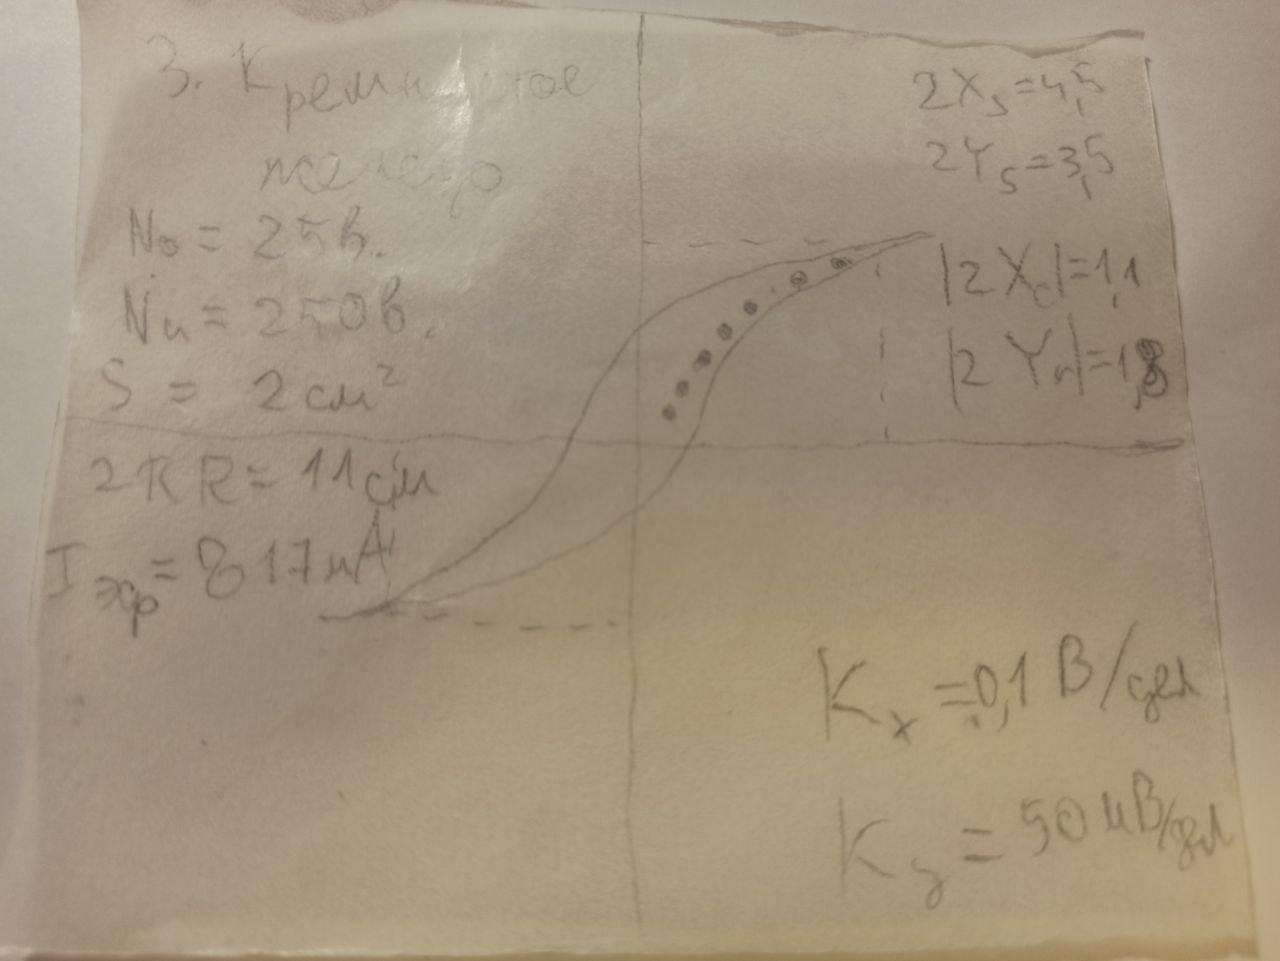
\includegraphics[scale = 0.15]{3}
    \centering
\end{figure}

\point Проведём калибровку горизонтальной оси ЭО. Для этого <<закоротим>> обмотку $N_0$ и подберём такой ток, при котором горизонтальная прямая занимает большую часть экрана. После чего найдём чувствительность канала по формуле:

\[
    K_{X-расч} = \frac{2R_0 \cdot \sqrt{2} \cdot I_{эф}}{2x}
\]

Из информации на установке можно узнать: $R_0 = 0,22~Ом$. Итого получаем:

\begin{align*}
    K_{X-ОЭ} &= 20~мВ & I_{эф} &= 290~мА & 2x &= 10 & K_{X-расч} &= 18~мВ \\
    K_{X-ОЭ} &= 50~мВ & I_{эф} &= 690~мА & 2x &= 9.7 & K_{X-расч} &= 44~мВ \\
    K_{X-ОЭ} &= 0,1~В & I_{эф} &= 1.4~А & 2x &= 9.7 & K_{X-расч} &= 89~мВ
\end{align*}

\point Разберём схему и измерим чувствительность канала $Y$ по формуле:

\[
    K_{Y-расч} = \frac{2\sqrt{2} \cdot U_{эф}}{2y}
\]

Результаты измерений приведены ниже:

\begin{align*}
    K_{Y-ОЭ} &= 20~мВ & U_{эф} &= 23~мВ & 2y &= 6.6 & K_{Y-расч} &= 10~мВ \\
    K_{Y-ОЭ} &= 50~мВ & U_{эф} &= 87~мВ & 2y &= 6.4 & K_{Y-расч} &= 38~мВ\\
\end{align*}

\point Найдём время интегрирующей цепочки. Для этого измерим её входное и выходное напряжение. $U_{вх} = 9,2 В$, $U_{вых} = 72~мВ$. Тогда получаем:

\[
    \tau = \frac{U_{вх}}{\omega \cdot U_{вых}} = 0,4~с
\]

\parag {Обработка результатов} ~\\

\point 

\begin{table}[!h]
    \centering
    \begin{tabular}{|c|c|c|c|c|c|c|}
    \hline
    Материал & $H$ & $B$ & $H_{max}$ & $B_s$ & $H_c$ & $B_r$ \\ \hline
    Феррит & 38 & 0.067 & 108 & 0.2 & 19 & 0.087 \\ \hline
    Пермаллой & 14 & 0.88 & 25.9 & 1.6 & 25.9 & 1.5 \\ \hline
    Кремнистое железо & 103 & 0.4 & 57 & 0.7 & 57 & 0.36 \\ \hline
    \end{tabular}
    \caption {Полученные характеристики для каждого материала}
    \label{V-A}
    \end{table}

\end {document}
